\documentclass[12pt]{article}
\usepackage[utf8]{inputenc}
\usepackage{amsmath, amssymb}
\usepackage{graphicx}
\usepackage{tikz}
\usepackage{pgfplots}
\usepackage{booktabs}
\usepackage{geometry}
\usepackage{textcomp}
\pgfplotsset{compat=1.18}

\geometry{margin=1in}

\begin{document}

% ===== PAGE 1 =====

\chapter*{\centering \textsc{Chapter 5}}
\section*{\centering \textsc{Confidence Intervals}}

The sample mean $\bar{X}$ and the sample variance $s^2$ provide estimates of the population mean $\mu$ and variance $\sigma^2$. They are called \emph{point estimators} because each provides a specific numerical value that is our best guess, based on the available data, of their parameter. We know that, as estimates, statistics are not necessarily going to be exactly equal to their parameters. Rather, we know that they vary from the parameters in a systematic fashion that is described by their sampling distributions. How close our estimate is to the parameter is not immediately known from the estimate itself. In this chapter we will consider \textbf{interval estimates} of the parameters. Rather than supplying a specific numerical value, intervals give us a range of plausible values for which we have some confidence that the parameter is contained.

\section*{\textsc{Confidence Interval for the Population Mean}}

Since the sample mean is based on a specific subset of a population it will reflect those scores which happen to be included in the sample. With a different sample there would be different scores and a different sample mean. The distribution of sample means drawn from a common population is called the \textbf{sampling distribution of the means}, and the variability of this distribution is measured by the \emph{variance of the means}, $\sigma_{\bar{X}}^2$, which is found by dividing the variance $\sigma^2$ by the sample size $n$ (see Formula 3.3). Our distance measure of the variability of sample means is the \emph{standard error of the means}, $\sigma_{\bar{X}}$, which is found by taking the square root of the variance of the means (see Formula 3.4).

If, for example, we randomly drew samples each based on $n=25$ observations from a population with $\mu=19$ and $\sigma^2=16$, we would have a sampling distribution of means centered at 19 with a standard error of:

\[
\sigma_{\bar{X}} = \sqrt{\sigma_{\bar{X}}^2} = \sqrt{\frac{16}{25}} = 0.80.
\]

With a sample size of $n=25$, the sampling distribution would closely approximate a normal curve, regardless of the shape of the original frequency distribution given what we learned about with the central limits theorem. The distribution would look much like Figure 5.1.

\begin{figure}[h]
\centering
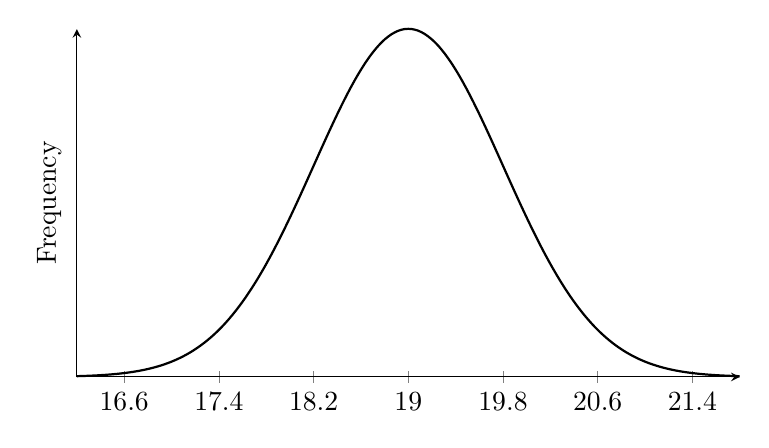
\begin{tikzpicture}
\begin{axis}[
    width=10cm,
    height=6cm,
    axis lines=left,
    xlabel={},
    ylabel={Frequency},
    xtick={16.6, 17.4, 18.2, 19.0, 19.8, 20.6, 21.4},
    ytick=\empty,
    xmin=16.2, xmax=21.8,
    ymin=0,
    domain=16.2:21.8,
    samples=100,
    clip=false,
]
\addplot[thick, black, smooth] {exp(-((x-19)^2)/(2*0.64))};
\end{axis}
\end{tikzpicture}
\caption*{\textbf{\emph{Figure 5.1}} \emph{Theoretical sampling distribution of sample means based on n=25.}}
\end{figure}

\newpage

% ===== PAGE 2 =====

Recall the special proportions (areas) under the normal curve that we learned in Chapter~2. Because our sampling distribution is assumed to be normal with a center at its parameter and a spread in standard errors (rather than standard deviations), we can infer that 68.26\% of the \textit{sample means} from the original population with a sample size of $n=25$ would fall between the values of 18.2 and 19.8 points (i.e., within $\pm 1$ standard error of $\mu=19$). Similarly, we can infer that 95.44\% of all sample means would fall within $\pm 2$ standard errors of the population mean. But if we wished to infer about the proportion of sample means falling within the \textit{exact} 95\% of the distribution (i.e., 47.50\% of each half of the curve), we'd use the Z-table to look up what z-score corresponded to .4750. We would find that the z-value corresponding to this proportion is 1.96. Hence, 95\% of the sample means would be within 1.96 standard errors of the population mean (i.e., ranging from a sample mean value of 17.43 up to a sample mean value of 20.57). It would indeed be very unusual to obtain a sample mean that is below 17.43 or above 20.57 points.

The rationale for developing an interval within which we expect to find the population mean is based on our knowledge of sampling distributions. Using the standard error of the mean, we can have some idea about how far \textit{sample means} based on a particular sample size are likely to vary from their parameter~$\mu$.

One of the primary lessons to learn about statistics is that we must learn to deal with some degree of uncertainty. In the case of the sample mean, we know that it usually falls fairly close to the parameter. Based on the table for the unit normal curve we know that 68.26\% are distributed within 1 standard error of the mean. If someone about to draw a sample asked what the value for their sample mean would be, I would be 68.26\% confident in guessing that it will be within 1 standard error of the population mean.

Continuing with our example, again, when we say that 68.26\% of the sample means fall between 18.2 and 19.8, it implies that we have a 68.26\% chance of drawing a single sample mean from the population with a value this close to the value of~$\mu$. If I wanted a better chance of forecasting what the value of a sample mean might be I would use a wider range. Specifically, there is \textit{exactly} a 95\% chance that any sample mean I draw at random from this sampling distribution will be 1.96 standard errors from~$\mu$. Thus I would have a 95\% chance of being correct if I guessed that the sample mean drawn at random would be somewhere between 17.43 and 20.57. I could continue to increase my belief, or confidence, that the sample mean will be within a specific range by continuing to increase the width of the range. However, if I wanted to be 100\% sure that an interval includes a specific, randomly chosen sample mean, I would have to make the interval width as wide as the entire spread of scores: I would have to include the possibility that the lowest values may be selected as well as the highest values. In effect, I would be admitting defeat with respect to forecasting what a likely sample mean would be because in theory, anything can happen. However, if we are willing to risk being wrong for some small percentage, we will be able to make an informed guess about what is likely to happen.

In statistics, we have to establish some probability that an inference (conclusion) that we make will be incorrect. Without this risk or uncertainty, we cannot provide any realistic limits. The most common level that we are willing to be wrong in the social sciences is 5\% (0.05); alternatively, the level that we will be correct is 95\% (0.95). A statement such as ``any random sample mean I draw will be between 17.43 and 20.57, with 95\% confidence'' is one that is clearly not assuming absolute certainty. There is the (small 5\%) possibility that the specific sample mean drawn will be filled with low scores and produce a mean lower than 17.43 or higher than 20.57. While this might happen, it is an

\newpage

% ===== PAGE 3 =====

extremely unlikely event. Of all the sample means that are possible, any sample mean
outside of the range of 17.43 and 20.57 will occur in only 5\% of the distribution (2.5\% in
each extreme).

The last paragraph discussed how we can forecast what values for the sample mean
will be found if we know the population mean and the standard error of the mean. More
commonly encountered is the reverse situation: one in which we know the value of one
sample mean from our research study and we wish to forecast what the plausible range for
the population mean is.

\textbf{\textit{A confidence interval is constructed to answer the question of: what values of a
parameter, such as $\mu$, are likely, given the statistic, such as the sample mean?}} For initial
learning purposes, we will assume that the true population standard error of the mean ($\sigma_{\bar{X}}$)
is somehow known to us. (This assumption will be relaxed soon.) While it would be
possible to construct 90\%, 99\%, or any other level confidence interval (by choosing the
appropriate z-score to include only that percentage of the sampling distribution), the social
sciences as a general discipline has nearly exclusively focused on the 95\% level; as such,
this is our focus. The general confidence interval (CI) formula for any parameter of interest,
assuming we know something about the true variance of the statistic, is given in Formula
5.1 below. Note that the interval is centered on the statistic and each `wing' (or ``margin of
error'') of the interval is the product of the statistic's standard error and the z-value
associated with the desired confidence level. The wings are termed ``margin of error''.

\begin{equation}
\text{CI} = \text{statistic} \pm \left( \text{z-value associated with \% of confidence level} \right)\!\left( \text{standard error} \right) \tag{5.1}
\end{equation}

\begin{center}
``wing'' or ``margin of error''
\end{center}

The 95\% confidence interval (95\%CI) for determining the location of the true
population mean, assuming we have the true variance available, is given in Formula 5.2,

\begin{equation}
95\%\text{CI} = \bar{X} \pm 1.96 \times \sigma_{\bar{X}} \tag{5.2}
\end{equation}

Imagine for the moment that we do not know the population mean for the
previously discussed sampling distribution of means shown in Figure 5.1. If a single sample
mean were found from this distribution, what might that sample mean be? It might be 18.9
or 19.2, or any other value. The primary point we learned in the last section was that most
of the sample means (95\% of them) will be within $\pm$1.96 standard errors of the population
mean. \textit{If we turn this statement inside-out, we know that the population mean is likely to be
within 1.96 standard errors of our sample mean.} The nice thing about distances such as the
standard error is that they work both ways. By knowing how far sample means tend to
vary from the population mean, we also know how far the population mean is likely to be
from the sample means. Only if we happen to have been as unfortunate as to have drawn
one of the most extreme 5\% of the possible sample means will the population mean not be
within $\pm$1.96 standard errors of the sample mean.

In our previous example the standard error of the mean $\sigma_{\bar{X}}$ was equal to 0.80 points.
Given this information, we know that 95\% of the sample means will be within
($\pm$1.96)*(0.80) = $\pm$1.568 points of the population mean $\mu$. Now imagine we had observed a
single sample of n=25 observations and had found that sample mean to be 18.5 points. We
would be able to make the inference that the true population mean $\mu$ was likely to be
within 1.568 points of the sample mean $\bar{X}$=18.5. Since we are pretending to not know the

\newpage

% ===== PAGE 4 =====

population mean, we would not know whether the specific estimate (the sample mean) we
obtained was an over- or under-estimate of the true mean $\mu$. To construct our interval we
would have to begin at 1.568 points below our sample mean of 18.5 and end at 1.568
points above our sample mean. Thus the lower bound (LB) of our interval would be $18.50 -
1.568 = 16.932$ points, and the upper bound (UB) of our interval would be $18.50 + 1.568 =
20.068$ points. We usually write this interval in brackets with the LB and UB separated by a
comma as: [16.932, 20.068]. Based on the information available to us, our best guess is that
the location of the population mean is contained in the interval of 16.932 to 20.068, with
95\% confidence. We add the clause of ``with 95\% confidence'' because of the way that we
constructed the interval (with a $z = 1.96$). We know that, of all the sample statistics that
might be drawn from a sampling distribution, 95\% of them are sufficiently close to their
respective parameter such that 95\% of all the intervals we could construct will contain the
parameter of interest. We call the interval a 95\% \textit{confidence interval} to indicate the level of
our belief in the truth of the interval.

The interval that we construct for a specific sample mean is a random variable and
will either be correct or incorrect: \textit{the parameter is either within that interval or it is not}.
Since in the real world we rarely know the parameter we will not know which of these two
possibilities happened for our constructed interval. Our probability statement refers to
what happens in the long-run. If the process of constructing a confidence interval were
repeated over and over again with different samples from the same population, each
interval would be different since it would be constructed about the different sample means.
This is what we mean by saying the interval (along with the sample mean) is a random
variable. What we know is that, of all the intervals that could be constructed, 95\% of them
will make a correct inference about the location of $\mu$. Note that in our example we can
actually evaluate the truth of our statement because we did in fact know the population
mean was 19 points. The interval of 16.932 to 20.068 points does include the value 19 in its
range, and thus it is a correct interval. If the sample which we had randomly drawn had
been one of the unusually small values possible, let's say 16.5 points, we would have
constructed an interval that extends from 14.432 to 18.068 points. We would have made a
similar statement as before but our interval range would reflect the low, rare value of a
sample mean that we happened to get: ``the true mean is located between 14.432 and
18.068 points, with 95\% confidence,'' but our interval would in truth be wrong. The price
we pay for making a guess about the location of a parameter based on the behavior of its
sampling distribution is that our guess can be wrong. Our solace is that we will only be
wrong when we draw a very unusual statistic from our sampling distribution -- something
that is very rare to occur. But such is the risk.

\section*{Confidence Interval with Unknown Variance}

In the preceding section we found the confidence interval for the population mean
when the true standard error of the mean $\sigma_{\bar{X}}$ was given to us. The true value of $\sigma_{\bar{X}}$ would
only be known when the true population variance $\sigma^2$ was available. The vast majority of
research does not have the true variance $\sigma^2$ available. Instead, we usually only have an
estimate of the variance, the sample variance $s^2$, which is computed using scores from our
subjects. Still, we'd like to be able to make a good guess of the location of $\mu$ using the
available information. With an unknown population variance, to construct our confidence
interval we will have to use an \textbf{estimated variance of the means} $s_{\bar{X}}^2$ (Formula 5.3) and an
\textbf{estimated standard error of the means} $s_{\bar{X}}$ (Formula 5.4) as follows.

\newpage

% ===== PAGE 5 =====

\begin{equation}
s_{\bar{X}}^2 = \frac{s^2}{n} \tag{5.3}
\end{equation}

\begin{equation}
s_{\bar{X}} = \sqrt{s_{\bar{X}}^2} = \sqrt{\frac{s^2}{n}} \tag{5.4}
\end{equation}

When the confidence interval for the population mean is computed using the estimated standard error rather than the true standard error, a slightly different procedure is required. The use of the statistic $s_{\bar{X}}$ introduces greater uncertainty into the total process of constructing a confidence interval. With the true variance known (i.e., when we have $\sigma_{\bar{X}}$) the only random variable involved in the confidence interval construction process is the sample mean. When the true variance is not known to us, we have added random variability due both to having to estimate the mean and the variance using our sample. The optional section of Chapter 4 indicates that sample variances also have random variability, just like sample means do. With more random variability involved due to having to estimate the variance, we have added uncertainty about the location of $\mu$. The defining characteristic of a 95\% confidence interval is that it is constructed in such a way that the statement that the population mean is within the interval will be true for 95\% of the possible samples that might be drawn. To reach the same level of confidence when the true variance is unknown, we will have to be more conservative in our construction process.

Specifically, when the standard error is computed using the estimated variance, particularly for smaller samples, we will have the concern that the sampling distribution will not be perfectly normally distributed and as such, the variance of the means could be underestimated. This would produce an estimated standard error $s_{\bar{X}}$ that was smaller than the true standard error $\sigma_{\bar{X}}$ and in turn underestimate the width of the confidence interval. An erroneously narrow interval would have less chance of containing $\mu$.

Figure 5.2 demonstrates this idea. Imagine we drew a single sample mean $\bar{X}$, drawn at random from a sampling distribution of means. Imagine that the sample mean is relatively high. Even though it turned out to be relatively high, if we constructed a 95\% confidence interval using the true standard error ($\sigma_{\bar{X}}$), we find that the interval that does (barely) contain the population mean $\mu$. However, if we did not have the true standard error available, and we instead estimated the standard error $s_{\bar{X}}$ using a sample that happened to have relatively little variability (i.e., a small sample variance), we would have an under-estimate of the true standard error $\sigma_{\bar{X}}$. So a confidence interval for the same sample mean (but using the \textit{estimated standard error}) would result in an interval that is slightly too narrow and misses the location of $\mu$.

\begin{figure}[ht]
\centering

\textbf{a. True population variance known.} By random sampling, a relatively high sample mean has been drawn, and $\mu$ is barely contained in the lower end of the interval.

\vspace{0.5em}

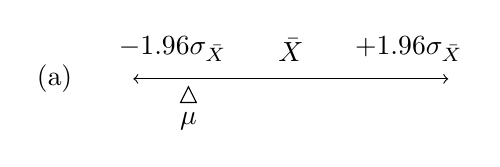
\begin{tikzpicture}
% Part (a)
\node at (-3, 0) {(a)};
\draw[<->] (-2, 0) -- (2, 0);
\node[above] at (-1.5, 0.1) {$-1.96\sigma_{\bar{X}}$};
\node[above] at (1.5, 0.1) {$+1.96\sigma_{\bar{X}}$};
\node[above] at (0, 0.1) {$\bar{X}$};
\draw (-1.4, -0.3) -- (-1.2, -0.3) -- (-1.3, -0.1) -- cycle;
\node[below] at (-1.3, -0.3) {$\mu$};
\end{tikzpicture}

\vspace{1em}

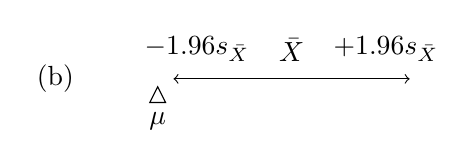
\begin{tikzpicture}
% Part (b)
\node at (-3, 0) {(b)};
\draw[<->] (-1.5, 0) -- (1.5, 0);
\node[above] at (-1.2, 0.1) {$-1.96s_{\bar{X}}$};
\node[above] at (1.2, 0.1) {$+1.96s_{\bar{X}}$};
\node[above] at (0, 0.1) {$\bar{X}$};
\draw (-1.8, -0.3) -- (-1.6, -0.3) -- (-1.7, -0.1) -- cycle;
\node[below] at (-1.7, -0.3) {$\mu$};
\end{tikzpicture}

\vspace{0.5em}

\textbf{b. Population variance unknown.} By random sampling, a relatively high sample mean and a moderately small sample variance have been drawn, $\mu$ is not contained within the interval.

\caption{Example of additional source of variability in intervals due to estimated variance.}
\label{fig:5.2}
\end{figure}

\newpage

% ===== PAGE 6 =====

Figure 5.2b illustrates the result if 1.96 (the z-value corresponding to the exact 47.5\% of the normal curve on either side of $\mu$) were multiplied with the estimated standard error. The failure of this interval to contain $\mu$ is the joint effect of the sample mean's value and the sample variance's value that we happened to have drawn. If we examined many samples drawn from a population with an estimated standard error we would actually find that there are more than 5\% of the intervals that would fail to contain $\mu$. The interval would not be a 95\% confidence interval but rather less than 95\%. In order to construct an interval that really has a 95\% chance of being correct we must widen the interval by multiplying the standard error by a value larger than the $z$=1.96. By going more than 1.96 standard errors in each direction, we can \textit{control for} the increased error associated with the random variability of having to use estimates for the mean and the variance.

The amount that we increase the multiplier is related to the extent that the standard error will vary from sample to sample. Imagine two extreme cases. In the first extreme case, the sample standard error is very unstable because it is based on a very few observations. The variance in Formula 5.1 would be based on very few degrees of freedom (i.e., a small sample) resulting in instability in our variance estimate. If it is unstable there is increased likelihood that the variance estimate will be considerably smaller than the parameter (the true variance), in turn producing a confidence interval that is much narrower than would have been found with the true standard error. In this case, the interval should be obtained by multiplying the standard error by a value considerably larger than 1.96. Note that the result of multiplying by a value greater than 1.96 will produce intervals that are much wider than before whenever the variance is overestimated. This unfortunate outcome cannot be avoided since we have no way of knowing whether the variance is an over or underestimate in reality.

In the second extreme case, imagine a sample that has many observations and thus a sample variance that is very stable and very similar to the population variance. The estimated standard error in this situation would be almost identical to the true standard error because the variance of the sample would be so like the population variance. There would be little need to have a greatly expanded multiplier to correctly produce a 95\% confidence interval: the multiplier would be only slightly bigger than 1.96.

Between these two extremes are all the values for the number of degrees of freedom on which the variance is based. The appropriate multiplier would depend on the specific number of degrees of freedom. As the number of degrees of freedom increases to infinity (we have infinite degrees of freedom when the true variance is known), the multiplier decreases until it reaches 1.96. The appropriate number of standard errors delineating the area of a sampling distribution that contains 95\% of its statistics based on a specific number of degrees of freedom is provided in the \textbf{\textit{t-table}} (in the appendix of the text).

The \textbf{\textit{t-distribution}} is a family of sampling distributions that model the distribution of statistics when the true variance is unknown. A t-curve is approximately normal in its shape, and in fact, becomes the unit normal curve (Z-distribution) when the true variance is known. In general, t-curves are shorter in the center and have thicker tails as compared with the normal z-curve (see Figure 5.3).

\newpage

% ===== PAGE 7 =====

\begin{figure}[ht]
\centering
\begin{tikzpicture}
  % Z distribution (solid line)
  \draw[thick, domain=-3.5:3.5, samples=100] plot (\x, {3.5*exp(-0.5*\x*\x)});
  % t-distribution (dotted line)
  \draw[thick, dotted, domain=-3.5:3.5, samples=100] plot (\x, {2.8*(1+\x*\x/3)^(-2)});
  % Axis
  \draw[->] (-4,0) -- (4,0) node[right] {\footnotesize (in standard errors)};
  % Mu label
  \node[below] at (0,0) {$\mu$};
  % Labels
  \node[above left] at (-0.3,3.5) {$Z$};
  \node[left] at (-1.8,2.2) {$t_{(df=n)}$};
\end{tikzpicture}
\caption{Comparison of Z distribution (solid line) with t-distribution (dotted line).}
\label{fig:5.3}
\end{figure}

We can determine the appropriate multiplier (the number of standard errors needed) for constructing a 95\% confidence interval that is based on the degrees of freedom associated with the estimated variance using this table. For this simple confidence interval for the true mean, our degrees of freedom are $df = n - 1$.

The first column of the t-table in the back of the book contains the number of degrees of freedom. In the remaining columns are the values of t that can be used as multipliers to contain different proportions of the curve. The proportions refer to the area of the curve that has numerical values more extreme than the t-value. To construct a 95\% confidence interval we would look under the column which has 5\% being more extreme than that value of t. The 5\% includes 2.5\% of the values in the t-curve that are greater than this positive value of t and 2.5\% that are smaller (lower) than the negative value of t. This type of presentation of the table is called a two-tailed table since the 5\% refers to the sum of two separate areas, one in each tail of the distribution. Figure~5.4 illustrates the critical values associated with the extreme 2.5\% of a t-distribution with $df = 10$.

\begin{figure}[ht]
\centering
\begin{tikzpicture}
  % t-distribution curve
  \draw[thick, domain=-3.5:3.5, samples=100] plot (\x, {3*exp(-0.5*\x*\x)});
  % Axis
  \draw[->] (-4,0) -- (4,0);
  % Mu label
  \node[below] at (0,0) {$\mu$};
  % Tick marks
  \foreach \x in {-3,-2,-1,1,2,3} {
    \draw (\x,0.1) -- (\x,-0.1) node[below] {\x};
  }
  % Shaded left tail
  \fill[pattern=north east lines] plot[domain=-3.5:-2.228, samples=50] (\x, {3*exp(-0.5*\x*\x)}) -- (-2.228,0) -- (-3.5,0) -- cycle;
  % Shaded right tail
  \fill[pattern=north east lines] plot[domain=2.228:3.5, samples=50] (\x, {3*exp(-0.5*\x*\x)}) -- (3.5,0) -- (2.228,0) -- cycle;
  % Labels for tail areas
  \node at (-2.8,0.5) {.025};
  \node at (2.8,0.5) {.025};
  % Critical value labels
  \node[below] at (-2.228,-0.4) {$t_{(10)} = -2.228$};
  \node[below] at (2.228,-0.4) {$t_{(10)} = 2.228$};
  % t_{(10)} label on curve
  \node[right] at (3,1.2) {$t_{(10)}$};
\end{tikzpicture}
\caption{Illustration of the critical values for a t-distribution with $df = 10$.}
\label{fig:5.4}
\end{figure}

\newpage

% ===== PAGE 8 =====

\section*{\textsc{Calculating the Confidence Interval}}

In the following two examples we illustrate the calculation of the confidence interval; in the first the population variance is known and in the second the population variance is not known, and distinguish between the procedure used with a known and an unknown population variance.

\subsection*{\textit{Situation: Known Population Variance}}

\hspace{1em} Imagine we have a sample of $n$=10 fourth grade reading scores as shown below.

\begin{center}
\textbf{X = \{15, 16, 17, 17, 18, 20, 21, 21, 22, 28\}}
\end{center}

Imagine further that we know the population variance of all fourth grade reading scores is $\sigma^2$=16. The 95\% confidence interval would be constructed using the normal curve's z-value that captures the exact 95\% of the distribution, which is 1.96. The 95\% CI formula would be as follows.

\begin{equation}
95\%\text{CI} = \bar{X} \pm 1.96 \cdot \sigma_{\bar{X}} \tag{from 5.2}
\end{equation}

If we calculate the sample mean we find that it turns out to be 19.5. As such, our confidence interval would be constructed as follows.

\begin{align*}
95\%\text{CI} &= 19.5 \pm 1.96 \cdot \sqrt{\frac{16}{10}} \\
95\%\text{CI} &= 19.5 \pm 1.96 \cdot \sqrt{1.6} \\
95\%\text{CI} &= 19.5 \pm 1.96 \cdot 1.265 \\
95\%\text{CI} &= 19.5 \pm 2.48 \\
95\%\text{CI} &= [19.5 - 2.48, \; 19.5 + 2.48] \\
95\%\text{CI} &= [17.02, \; 21.98]
\end{align*}

Our final statement is: ``the population mean $\mu$ is between 17.02 and 21.98, with 95\% confidence.''

\subsection*{\textit{Situation: Unknown Population Variance}}

\hspace{1em} Let us return to the sample of $n$=10 fourth-grade scores, but now let's assume that the true variance $\sigma^2$ is \textit{not} known to us. Instead, we must estimate the variance. Thus, we will need to compute not only the sample mean, but also the sample variance. Further, we will need to compute our confidence interval using a t-value based on $n-1$ degrees of freedom (in our case, $df$=9), rather than a z-value. The formula for computing the confidence interval when the true variance is unknown is as follows. (Formula 5.4 provides the formula for computing the estimated standard error of the means).

\begin{equation}
95\%\text{CI} = \bar{X} \pm t_{(df=n-1)} \cdot s_{\bar{X}} \tag{5.5}
\end{equation}

The first order of business is that we must compute the sample variance. The sample mean was already computed earlier and found to be 19.5. Recall from Chapter 4 that the estimated variance is computed as $s^2 = (\Sigma(X - \bar{X})^2)/(n-1)$, or in other words, the sum of the squared deviations (SS) divided by the degrees of freedom (df). Below are the estimates.

\newpage

% ===== PAGE 9 =====

\begin{center}
\begin{tabular}{c c c}
\hline
$X$ & $(X - \bar{X})$ & $(X - \bar{X})^2$ \\
\hline
15 & $15 - 19.5 = -4.5$ & $(-4.5)^2 = 20.25$ \\
16 & $-3.5$ & 12.25 \\
17 & $-2.5$ & 6.25 \\
17 & $-2.5$ & 6.25 \\
18 & $-1.5$ & 2.25 \\
20 & 0.5 & 0.25 \\
21 & 1.5 & 2.25 \\
21 & 1.5 & 2.25 \\
22 & 2.5 & 6.25 \\
28 & 8.5 & 72.25 \\
\hline
\textbf{SUMS} & \textbf{195} \quad \textbf{0} & \textbf{130.5} \\
\hline
\end{tabular}
\end{center}

\[
\bar{X} = \frac{\sum X}{n} \qquad s^2 = \frac{\sum (X - \bar{X})^2}{n - 1}
\]
\[
\bar{X} = \frac{195}{10} \qquad s^2 = \frac{130.5}{10 - 1}
\]
\[
\bar{X} = 19.5 \qquad s^2 = 14.5
\]

From the computations above, we see that the sample variance, $s^2$, is 14.5. Next, we look up
the t-value (in the back of the text) corresponding to $\text{df}=9$. In the row for $\text{df}=9$, we move to
the right to the column labeled 0.05. The entry in the row for this column is 2.262. Now we
can compute our interval as follows.

\[
95\%\text{CI} = \bar{X} \pm t_{(\text{df}=n-1)} \cdot s_{\bar{X}}
\]
\[
95\%\text{CI} = 19.5 \pm 2.262 \cdot \sqrt{\frac{14.5}{10}}
\]
\[
95\%\text{CI} = 19.5 \pm 2.262 \cdot \sqrt{1.45}
\]
\[
95\%\text{CI} = 19.5 \pm 2.262 \cdot 1.204
\]
\[
95\%\text{CI} = 19.5 \pm 2.72
\]
\[
95\%\text{CI} = [19.5 - 2.72, \; 19.5 + 2.72]
\]
\[
95\%\text{CI} = [16.78, \; 22.22]
\]

Based on the available information this represents the interval within which we
have 95\% confidence that the parameter is contained. In this example the interval is
broader than the interval we constructed when the population variance was known. With
less information we are less sure of our estimates and often end up with wider intervals.
We need this additional width to maintain our overall chance of being correct in our
inference about $\mu$.

The most difficult point to master with respect to confidence intervals is the
meaning of the probability statement. Specifically, when we say there is a 95\% chance that
the population mean is contained within the interval, to what does the 95\% refer? To
understand this statement we must recall that the population mean is a constant. It is
assumed to have a numerical value which is independent of the selection of the sample.
There are an infinite number of possible samples from a population but regardless which
one is drawn, the population mean is the same. The sample mean will change from sample

\newpage

% ===== PAGE 10 =====

\section*{\textsc{Confidence Interval for the Variance (Optional)}}

A confidence interval can be constructed using any statistic that has a known sampling distribution. We have dwelt on the confidence interval for the population mean because this is typically the most important description of a population. In the present section we will briefly discuss the procedures for establishing a confidence interval for a population variance. Because the sampling distribution of the variances is not symmetric for the lower number of degrees of freedom, the procedures used differ considerably.

At the end of Chapter 4 (optional section) we discussed the sampling distribution of the variances. It was a skewed distribution whose shape became more symmetric as the degrees of freedom increased. The $\chi^2$ distribution described the distribution of a linear transformation of the sample variance. The transformation was as follows.

\[
\chi^2 = \frac{(n-1)(s^2)}{\sigma^2} \quad \text{with } df = n - 1
\]

From the $\chi^2$ distribution we can determine how large or small the value of $\chi^2$ would be before that value was one of the most extreme 5\%. All values of $\chi^2$ between these two values would be the middle most 95\% of the values of $\chi^2$ which happen when random samples are drawn from a population. Since the value of $\chi^2$ is a function of the sample variance, the population variance and the sample size, we could obtain possible values for the population variance which would produce values of $\chi^2$ which would be consistent with sample variance and sample size.

The variance for our 10 scores in the example in this chapter turned out to be $s^2 = 14.5$. Our question is within what range is the location of the population variance $\sigma^2$? With 9 degrees of freedom, we find from the $\chi^2$ distribution (given in the back of the book) that 2.5\% of the values of $\chi^2$ have values smaller than 2.7 or larger than 19.0. Using the equation for $\chi^2$ we know that the degrees of freedom ($n - 1 = 9$) multiplied by the ratio of the estimated variance to the population variance will seldom be smaller than 2.7 or larger than 19.0. If our sample variance is $s^2 = 14.5$, what values for $\sigma^2$ would produce these extreme values for $\chi^2$? Rearranging the terms in the $\chi^2$-equation we have:

\[
\chi^2 = \frac{(n-1)(s^2)}{\sigma^2} \qquad \equiv \qquad \sigma^2 = \frac{(n-1)(s^2)}{\chi^2}
\]

The lower bound (LB) of a confidence interval would be that value of $\sigma^2$ which produces the maximum expected value of $\chi^2$:

\[
\text{LB} = \frac{(10-1)(14.5)}{19.023} = \frac{130.5}{19.023} = 6.86.
\]

And the upper bound (UB) for $\sigma^2$ would be that which produces the lowest $\chi^2$:

\newpage

% ===== PAGE 11 =====

\[
\text{UB} = \frac{(10-1)(14.5)}{z^2} = \frac{130.5}{z^2} = 48.33.
\]

Thus our 95\% confidence interval for the population variance is 6.86 to 48.33. The interval we constructed contains all the values of $\sigma^2$ that would be expected to produce a sample variance of 14.5. If the population variance is in truth less than 6.86 or greater than 48.33, then our sample variance is unexpectedly large or small, respectively. Whatever the true variance really is, we know that 5\% of the sample variances we could ever compute will be in these extremes, and for these rare estimates, our interval will not contain the parameter.

The interval we constructed has a 95\% chance of correctly containing $\sigma^2$. There are other intervals for this sample that would also have a long-run expectation of being correct. We could of course use a different level of confidence and as such our interval can be wider (higher confidence) or narrower (lower confidence). Of all the possible confidence levels we could use, we have to decide on which is best. Typically we want a narrower interval so that we can be more precise about our guess of the location of the parameter. However, we don't want to be wrong very often either. In the social sciences, the 95\% confidence level was somewhat arbitrarily chosen a long time ago as a good level of precision without much risk for being wrong.

With sample variances, the sampling distribution is not symmetric and the shortest range is not found by taking 2.5\% at the bottom and the top of a distribution as we do with sampling distributions of means (which are normally or close to normally distributed). The shortest width of a confidence interval for a variance depends on the amount of skew in its sampling distribution which, in turn, depends on the number of degrees of freedom used to estimate the variance. Nevertheless, using the procedure discussed above will provide an interval that is sufficiently close to reality, particularly as $\chi^2$ becomes more symmetric.

\newpage

% ===== PAGE 12 =====

\section*{\textsc{Practice Exercises}}

\begin{enumerate}
\item Imagine you have a sample mean of $\bar{X}=20.8$ and you know that the \textit{true} standard error of the mean $\sigma_{\bar{X}}=3.7$. Compute the 95\% confidence interval.

\item Imagine that you have a sample mean of $\bar{X}=105.2$ and you know that the \textit{true} standard error of the mean $\sigma_{\bar{X}}=15.6$. Compute the 95\% confidence interval.

\item Imagine that you have a sample mean of $\bar{X}=72.1$ and you only have the \textit{estimated} standard error of the mean $s_{\bar{X}}=13.5$. Your sample size for your estimated mean and variance is $n=15$. Compute the 95\% confidence interval.

\item Imagine that you have a sample mean of $\bar{X}=209.3$ and you only have the \textit{estimated} standard error of the mean $s_{\bar{X}}=22.5$. Your sample size for your estimated mean and variance is $n=30$. Compute the 95\% confidence interval.
\end{enumerate}

\newpage

% ===== PAGE 13 =====

\section*{\textsc{Answers to Practice Exercises}}

\begin{enumerate}
    \item 95\%CI = [13.55,\ \ 28.05]. The true mean is between 13.55 and 28.05, with 95\% confidence. \textit{Note: the critical value or multiplier to use in this problem is $z$=1.96.}
    \item 95\%CI = [74.62,\ \ 135.78]. The true mean is between 74.62 and 135.78, with 95\% confidence. \textit{Note: the critical value or multiplier to use in this problem is $z$=1.96.}
    \item 95\%CI = [43.14,\ \ 101.06]. The true mean is between 43.14 and 101.06, with 95\% confidence. \textit{Note: the critical value or multiplier to use in this problem is $t_{(df=14)}$=2.145.}
    \item 95\%CI = [163.29,\ \ 255.31]. The true mean is between 163.29 and 255.31, with 95\% confidence. \textit{Note: the critical value or multiplier to use in this problem is $t_{(df=29)}$=2.045.}
\end{enumerate}

\end{document}
